\documentclass[a4paper, 12pt]{article}

\usepackage[top=2cm, bottom=2cm, left=2.5cm, right=2.5cm]{geometry}
\usepackage[utf8]{inputenc}
\usepackage{array}
\usepackage{graphicx}

\graphicspath{{img/}}

\begin{document}
\begin{flushleft}
\includegraphics{logo}\\
\textbf{UNIVERSIDADE ESTADUAL DE PONTA GROSSA} \\
SISTEMA UNIVERSIDADE ABERTA DO BRASIL - UAB \\
\underline{Licenciatura em Matemática | Polo UAB em Jacarezinho}\end{flushleft} 
\textbf{ALUNO:} Ricardo Medeiros da Costa Junior   \textbf{RA:} 151774301 \\
\textbf{DISCIPLINA:} 101505 - Cálculo Diferencial e Integral II \\
\textbf{ATIVIDADE:} Tarefa - Unidade II (Valor: 5 pontos) \\
\textbf{TUTOR(A):} Adilane de Assis Ferreira \\
\textbf{PERÍODO:} Quarto Período \\
\begin{enumerate}
\item ({\it Valor: 0,05 pontos de cada}) Calcule as seguintes integrais:
  \begin{enumerate}
  \item $ \int \! \frac{x^{5}+x+1}{x^{2}} \, \mathrm{d}x $
\begin{figure}[h!]
  \centering
  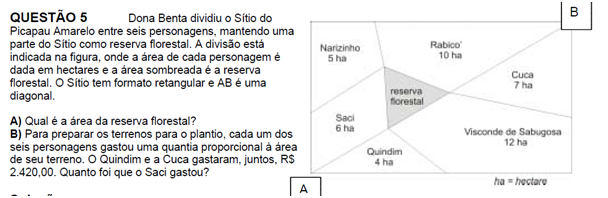
\includegraphics[width=0.7\textwidth]{1}
\end{figure} 
    
  \item $ \int \! \left ( \frac{3}{x} + \frac{2}{x^{3}} \right ) \, \mathrm{d}x $\begin{figure}[h!]
  \centering
  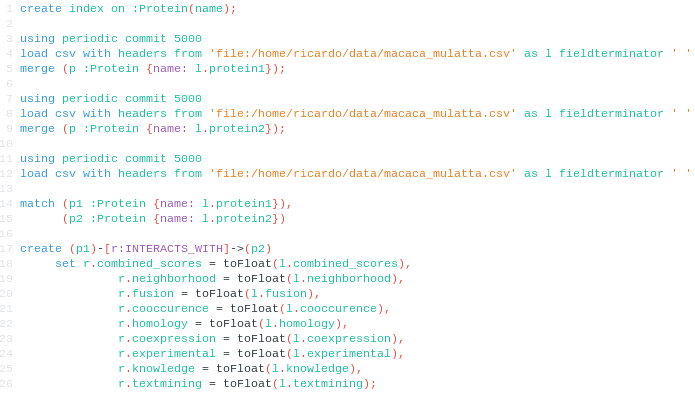
\includegraphics[width=0.7\textwidth]{2}
\end{figure} 

  \item $ \int \! \left ( \sqrt[3]{x} - \frac{1}{2 \sqrt[3]{x}} \right ) \, \mathrm{d}x $\begin{figure}[h!]
  \centering
  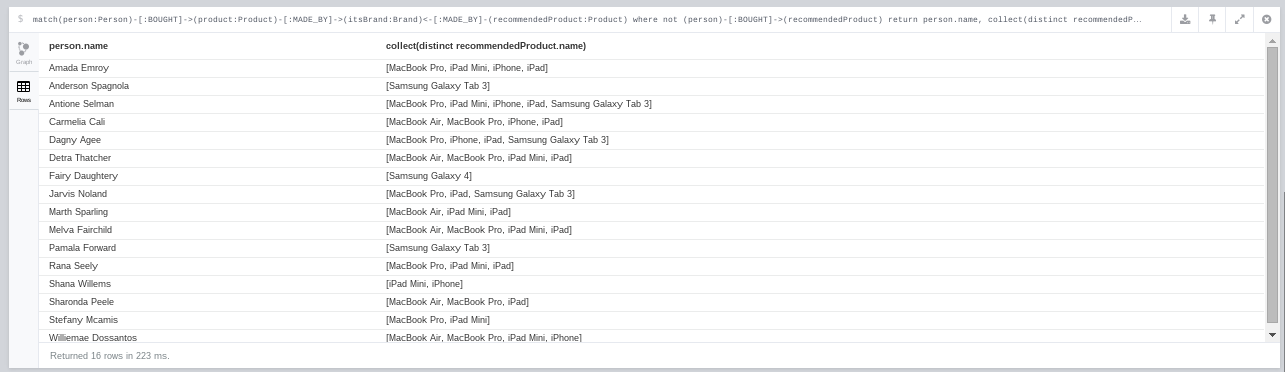
\includegraphics[width=0.7\textwidth]{3}
\end{figure} 

  \item $ \int \! \mathrm{sen}(3x) \, \mathrm{d}x $
    \begin{figure}[h!]
  \centering
  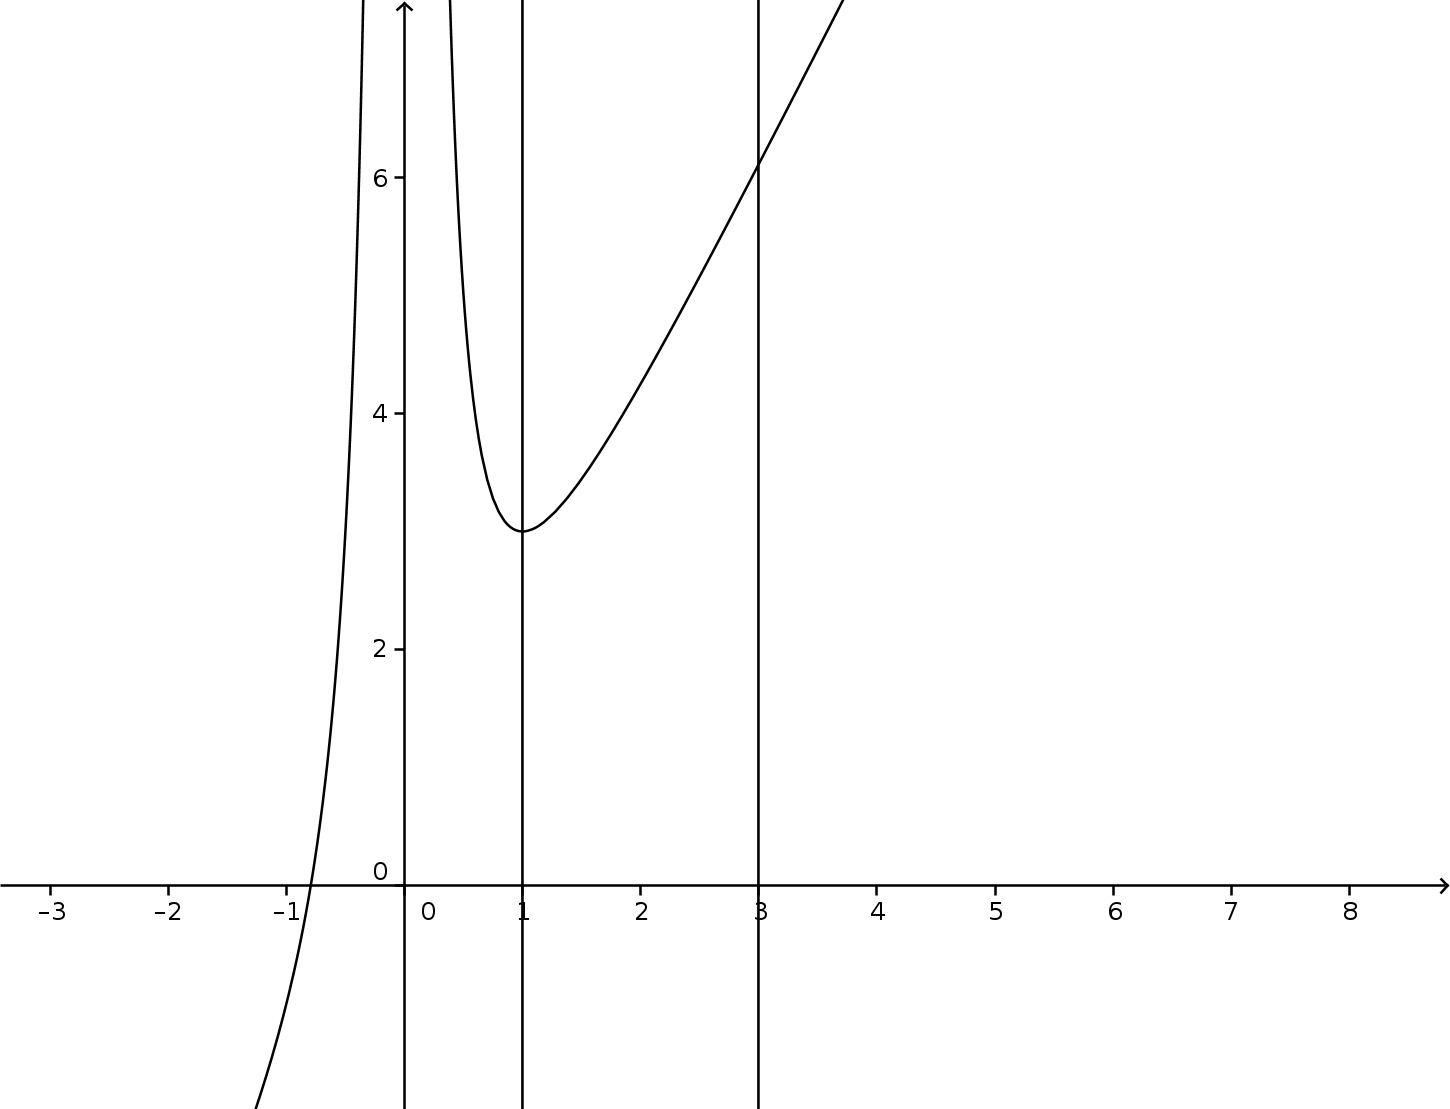
\includegraphics[width=0.7\textwidth]{4}
\end{figure} 

  \item $ \int \! \frac{1+4x}{\sqrt{1+x+2x^{2}}} \, \mathrm{d}x $
    \begin{figure}[h!]
  \centering
  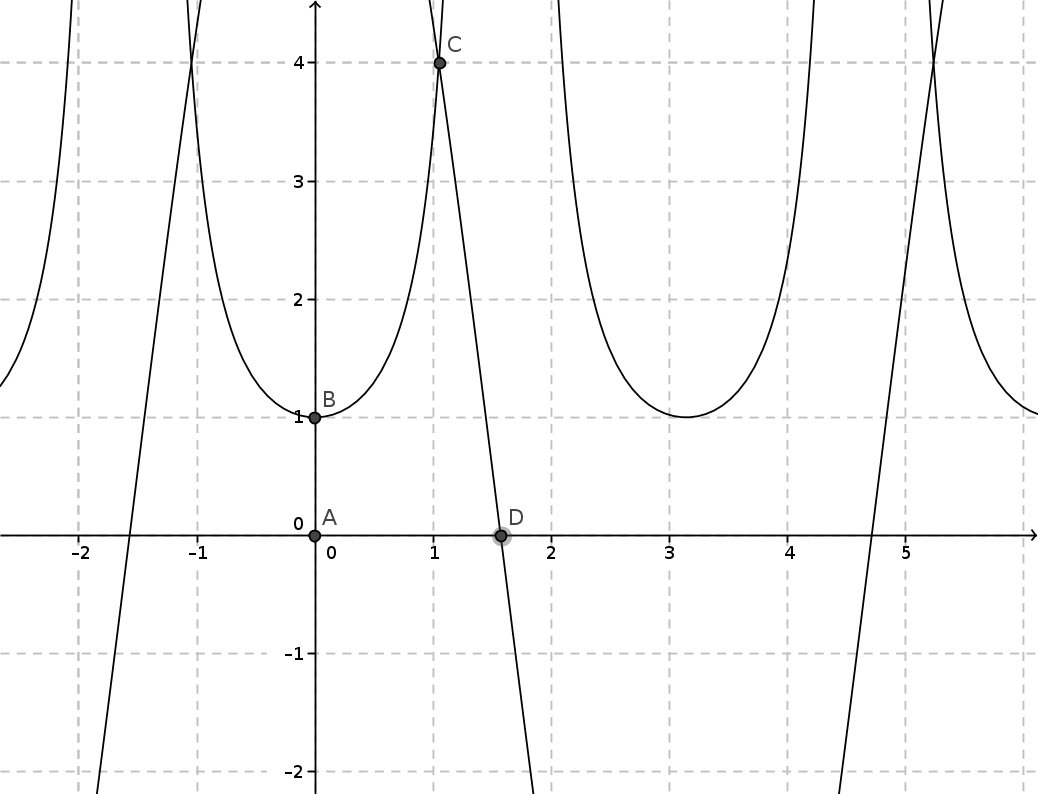
\includegraphics[width=0.7\textwidth]{5}
\end{figure} 

  \item $ \int \! \frac{1+x}{1+x^{2}} \, \mathrm{d}x $
  \item $ \int \! \mathrm{cos}^{4} \left( \frac{x}{2} \right) \mathrm{sen} \left(\frac{x}{2} \right) \, \mathrm{d}x $
  \item $ \int \! \frac{4x+6}{(x^{2}+3x+7)^{3}} \, \mathrm{d}x $
  \item $ \int \! 7^{\mathrm{cos}(9x)} \mathrm{sen}(9x) \, \mathrm{d}x $
  \item $ \int \! \mathrm{tg}^{2} \left( \frac{4x}{3} \right) \mathrm{sec}^{2} \left(\frac{4x}{3} \right) \, \mathrm{d}x $    
  \end{enumerate}
\end{enumerate}
\end{document}
